%\documentclass[12pt]{article}
\documentclass[12pt]{report}

%% Escrevendo em português
\usepackage[brazil]{babel}
\usepackage[utf8]{inputenc}
%\usepackage[latin1]{inputenc}
%\usepackage{isolatin1}
 %% Figuras  eps
\usepackage{graphicx}
\usepackage{xcolor}

\usepackage{amsfonts}
\usepackage{amsthm}
\usepackage{mathtools}
%%para inserir figuras lado a lado
% \usepackage{subfig} Dá erro
\usepackage{caption}
\usepackage{subcaption}

%usa a, b, c ... em enumerate
%\usepackage{enumitem}
\usepackage{enumerate}
\usepackage{afterpage}
\usepackage{url}

\usepackage[T1]{fontenc}
\usepackage[utf8]{inputenc}
\usepackage{mathtools}   % loads »amsmath
\usepackage[portuguese, ruled, linesnumbered]{algorithm2e}

\usepackage{longtable}
%% Pulando linhas
\renewcommand{\baselinestretch}{1.5}

\newcommand{\vsp}{\vspace{0.2in}}

\newcommand{\beq}{\begin{equation}} 
\newcommand{\eeq}{\end{equation}} 
\newcommand{\beqa}{\begin{eqnarray}} 
\newcommand{\eeqa}{\end{eqnarray}} 
\newcommand{\bfga}{\begin{figure*}} 
\newcommand{\efga}{\end{figure*}} 
\newcommand{\bfg}{\begin{figure}} 
\newcommand{\efg}{\end{figure}} 
\newcommand{\etal}{{\it et al.}} 
\newcommand{\aluno}{{ Rafael Pereira Lima}}
\newcommand{\link}{\textit{link}} 
\newcommand{\links}{\textit{links}} 



\newcommand{\argmin}{\operatornamewithlimits{argmin}}
\newcommand{\argmax}{\operatornamewithlimits{argmax}}

%\usepackage[fapesp]

% Tamanho da página
\setlength{\textwidth}{6.5in}
\setlength{\textheight}{8.5in}

% Parágrafo
\setlength{\parindent}{5mm}
\setlength{\parskip}{1mm}

% Empurra para cá empurra para lá
\evensidemargin -0.3cm
\oddsidemargin -0.3cm
\topmargin -0.7in

\newtheorem{definicao}{Definição}
\newtheorem{proposicao}{Proposição}
\newtheorem{lema}{Lema}
\newtheorem{corolario}{Colorário}
\newtheorem{teorema}{Teorema}

\begin {document}

% ---------------------------------------------------------------------------- %
% CAPA
\thispagestyle{empty}
\begin{center}
    \vspace*{2.3cm}
    Universidade de São Paulo\\
    Instituto de Matemática e Estatística\\
    Matemática Aplicada - Bacharelado - Habilitação em Métodos Matemáticos


    \vspace*{3cm}
    \Large{Rafael Pereira Lima}
    

    \vspace{3cm}
    \textbf{\Large{Rastreamento de Olhar Usando Compressive Sensing}}
    
       
    \vskip 5cm
    \normalsize{São Paulo}

    \normalsize{Dezembro de 2016}
\end{center}

% ---------------------------------------------------------------------------- %
% Página de rosto
%
\newpage
\thispagestyle{empty}
    \begin{center}
        \vspace*{2.3 cm}
        \textbf{\Large{Rastreamento de Olhar Usando Compressive Sensing}}
        \vspace*{2 cm}
    \end{center}

    \vskip 2cm

    \begin{flushright}
	Monografia final da disciplina \\
        MAP2080 -- Trabalho de Formatura.
    \end{flushright}

    \vskip 5cm

    \begin{center}
    Supervisor: Prof. Dr. Carlos Hitoshi Morimoto\\
%    $[$ Cosupervisor: Prof. Dr. Nome do Cosupervisor $]$

%    \vskip 5cm
    \vskip 4.5cm
    \normalsize{São Paulo}
    
    \normalsize{Dezembro de 2016}
    \end{center}
\pagebreak
% ---------------------------------------------------------------------------- %

% Resumo
\chapter*{Resumo}

Informações do olhar podem ser usadas para melhorar a experiência do usuário ou possibilitar a interação com o computador quando, por limitações físicas, a pessoa é incapaz de interagir com dispositivos de entrada usuais. Rastreamento de olhar consiste na identificação da posição do olhar durante determinado período. Desenvolvemos um programa de rastreamento de olhar usando \textit{Compressive Sensing}, uma técnica usada para recuperar sinais esparsos. Os resultados obtidos foram semelhantes aos presentes na literatura.

\noindent \textbf{Palavras-chave:} \textit{Compressive Sensing}, rastreamento de olhar, processamento de imagens.

%Elemento obrigatório, constituído de uma sequência de frases concisas e objetivas, em forma de texto.  Deve apresentar os objetivos, métodos empregados, resultados e conclusões.  O resumo deve ser redigido em parágrafo único, conter no máximo 500 palavras e ser seguido dos termos representativos do conteúdo do trabalho (palavras-chave).

% ---------------------------------------------------------------------------- %

% ---------------------------------------------------------------------------- %
% Abstract
\chapter*{Abstract}

Gaze information can be used to improve user experience or enable human-computer interaction when the person is unable to use common input devices due to physical disabilities. Gaze tracking is the gaze position estimation in some period of time.  We developed a gaze tracking algorithm with Compressive Sensing, a technique used to recover sparse signals. The results are similar to those in the literature.

\noindent \textbf{Keywords:} Compressive Sensing, gaze tracking, image processing.

% ---------------------------------------------------------------------------- %
% Sumário
\tableofcontents    % imprime o sumário

\chapter{Introdução}

Um dos problemas enfrentados por pessoas com deficiência motora é a falta de acesso à informação devido à impossibilidade ou dificuldade para usar dispositivos eletrônicos. Uma possível solução para esse problema seria usar o movimento dos olhos para interagir com o mundo exterior. O uso de técnicas para identificar onde determinada pessoa está olhando é chamado de rastreamento de olhar.

Para rastrear o olhar geralmente uma câmera é posicionada na frente de um dos olhos. A partir da imagem obtida pela câmera, técnicas de processamento de imagens são usadas para identificar a posição da íris e, a partir disso, identificar a direção em que o usuário está olhando. No entanto, o rastreamento de olhar é dificultado por vários fatores, como mudanças na iluminação do lugar e oclusão parcial dos olhos causada por alguma expressão facial. Portanto, não é uma tarefa trivial mas, apesar dessas dificuldades, deve ser executada em tempo real.

Uma possível solução seria processar não a imagem original, mas uma imagem menor e com as mesmas características desejadas encontradas na primeira.

Uma imagem pode ser representada como uma combinação linear de vetores que representam senoides de frequências diferentes. Empiricamente é assumido que frequências mais altas influenciam pouco no resultado final e, por esse motivo, em muitas aplicações essas frequências são descartadas para compressão de imagens, ou seja, reduzir o 'espaço físico' usado para armazenar o arquivo.

A abordagem sugerida pelo Compressive Sensing (CS) é um pouco diferente: em vez de assumir quais vetores podem ser descartados, é assumido que uma determinada quantidade de vetores exerce pouca ou nenhuma influência no sinal. Chamamos de esparso um sinal que depende apenas de uma pequena quantidade de vetores da base. Quando o sinal depende de vários vetores, porém apenas uma pequena quantidade influencia significativamente no resultado final, esse sinal é conhecido como `compressive'. Em muitos casos CS permite reconstruir, sem perda de qualidade, uma imagem usando menos amostras do que as necessárias para reconstruir imagens usando técnicas tradicionais de compressão de imagens.
\chapter{Rastreamento de olhar}

%Rastreamento de olhar consiste em técnicas para determinar a direção do olhar, ou seja, a partir da posição da íris identificar para onde uma pessoa está olhando.

Rastreamento de olhar consiste em determinar a direção do olhar, ou seja, a partir da posição do olho identificar para onde uma pessoa está olhando em determinado instante e também mudanças na direção do olhar em determinado período \cite{lupung}.

Abaixo listamos algumas aplicações de rastreamento de olhar.

\section{Aplicações}

Podemos usar o rastreamento de olhar para construir interfaces para ajudar pessoas com dificuldades motoras a interagir com computadores \cite{lidade}. \newc{Kurauchi et al.\cite{kurauchi2016eyeswipe} desenvolveram} um teclado virtual que permite a digitação através do olhar, como mostra a Figura $\ref{fig:eyeswipe}$.

\begin{figure}
\centering
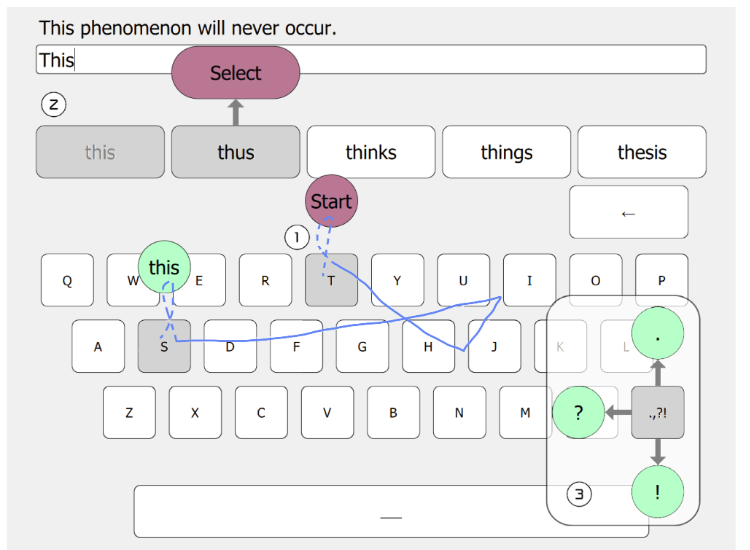
\includegraphics[scale=.3]{imagens/teclado.png}
\caption{Um teclado virtual controlado pelo olhar permite a interação de pessoas com dificuldades motoras com o computador. Reproduzido de \cite{kurauchi2016eyeswipe}.}
\label{fig:eyeswipe}
\end{figure}

Através da análise da posição do olhar é possível avaliar a influência de um anúncio sobre a atenção dos consumidores e, assim, ajudar na criação de propagandas mais eficientes \cite{duchowski2002breadth}. A Figura \ref{fig:propaganda} mostra as regiões onde as pessoas mais prestam atenção ao observar um anúncio.

\afterpage{
\begin{figure}
\begin{center}
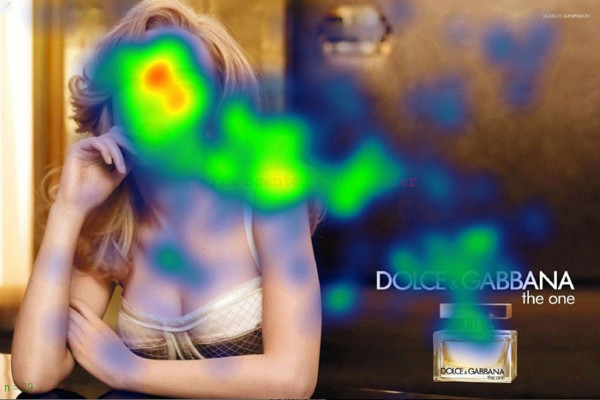
\includegraphics[scale=.4]{imagens/dolcegabbana_heatmap.jpg}
\caption[]{O rastreamento de olhar pode ser usado para a avaliar a eficiência de uma propaganda. Regiões coloridas indicam onde as pessoas prestam mais atenção no anúncio. Reproduzido de \protect \small{\url{http://www.businessinsider.com.au/eye-tracking-heatmaps-2014-7}}}
\label{fig:propaganda}
\end{center}
\end{figure}
%\footnotetext{\url{http://www.businessinsider.com.au/eye-tracking-heatmaps-2014-7}}
}

O olhar também pode ser usado como um indicador de usabilidade de interfaces de \textit{software}, sendo usado em estudos de interação humano-computador (IHC) \cite{duchowski2002breadth}. Um estudo feito por \cite{nielsen2007fancy} mostra que usuários tendem \newc{a} ignorar informações que parecem propagandas em um site. No caso, solicitaram para os participantes encontrarem a população dos Estados Unidos e $86\%$ dos participantes falharam, mesmo com o número localizado no topo da página e escrito em vermelho. A Figura $\ref{fig:censo}$ mostra as regiões mais observadas pelos usuários.

%\begin{figure}
%\begin{center}
%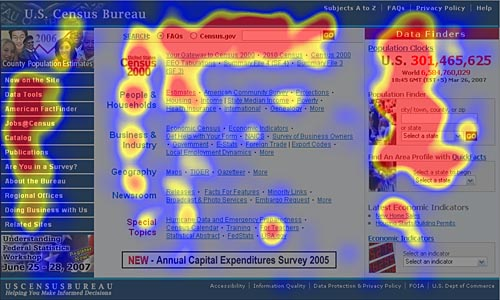
\includegraphics[scale=.7]{imagens/census-homepage-heatmap.jpg}
%\caption{Regiões vermelhas são as mais observadas no site por participantes procurando a população dos Estados Unidos. Note que a região com essa informação, no canto superior direito, é parcipalmente observada, indicando que foi ignorada pelos usuários. Reproduzido de \cite{nielsen2007fancy}.}
%\label{fig:censo}
%\end{center}
%\end{figure}

\afterpage{
\begin{figure}
\centering
	\begin{subfigure}[b]{1\textwidth}
		\centering
		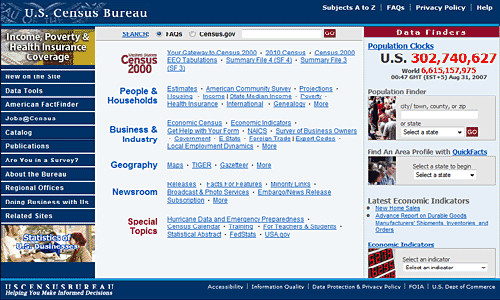
\includegraphics[scale=.7]{imagens/census-homepage-small.jpg}
		\caption{}
	\end{subfigure}\\
	\begin{subfigure}[b]{1\textwidth}
		\centering
		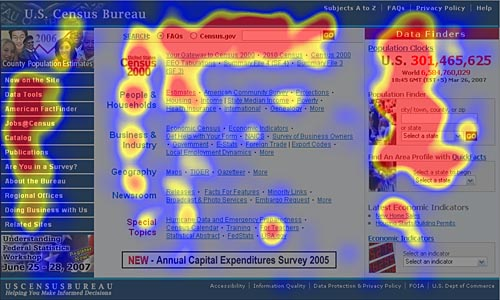
\includegraphics[scale=.7]{imagens/census-homepage-heatmap.jpg}
		\caption{}
	\end{subfigure}
	\caption{\newc{{\bf a} Imagem original do site. Regiões vermelhas em {\bf (b)}} são as mais observadas no site por participantes procurando a população dos Estados Unidos. Note que a região com essa informação, no canto superior direito, é parcipalmente observada, indicando que foi ignorada pelos usuários. Reproduzido de \cite{nielsen2007fancy}.}
	\label{fig:censo}
\end{figure}
%\footnotetext{\url{http://www.businessinsider.com.au/eye-tracking-heatmaps-2014-7}}
}
\section{Técnicas de rastreamento de olhar}

Técnicas de rastreamento de olhar determinam a posição do olhar a partir do movimento dos olhos. Algumas partes do olho humano, que estão representadas na Figura $\ref{fig:olho}$,  são as seguintes \cite{lidade}:

\afterpage{
%assim o footnote funciona http://blog.peschla.net/2012/11/latex-footnotes-in-captions/
\begin{figure}
\begin{center}
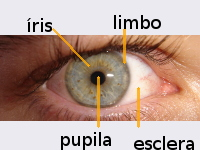
\includegraphics[scale=1]{imagens/eye.jpg}
\caption[]{Regiões do olho. Adaptado de \protect \small{\url{http://commons.wikimedia.org/wiki/File:My_eye.jpg}}}
\label{fig:olho}
\end{center}
\end{figure}
%\footnotetext{\url{http://commons.wikimedia.org/wiki/File:My_eye.jpg}}
}

\begin{itemize}
\item \textbf{pupila}: a abertura que permite a entrada de luz no olho.
\item \textbf{íris}: o músculo colorido que controla o diâmetro da pupila.
\item \textbf{esclera}: tecido branco protetor que envolve o restante do olho.
\item \textbf{limbo}: o contorno entre a íris e a esclera.
\end{itemize}

%[sic: no texto estava Eye location/tracking techniques can be...]
%Técnicas de rastreamento de olhar podem ser divididas em três modalidades \cite{valenti2009webcam}.

~ %para evitar um erro estranho de missing item

Técnicas de rastreamento de olhar podem ser divididas em três modalidades \cite{valenti2009webcam}:

\begin{enumerate}
\item {\bf Eletro-oculografia}, que registra diferenças de potencial elétrico na pele ao redor da cavidade ocular.
\item {\bf Lente de contato}, uma bobina é instalada no olho sobre uma lente de contato e a posição do olho é estimada ao medir o campo eletromagnético. \cite{duchowski2007eye}. Este método é o mais preciso para medir movimentos do olho, porém é o mais \oldc{invasivo}\newc{desconfortável} \cite{duchowski2007eye}.

%sic: no texto estava oculografia baseada em foto ou vídeo
\item  {\bf Rastreamento baseado em vídeo}, que usa técnicas de processamento de imagens para identificar a posição da pupila nas imagens do olho. \newc{Esse método é mais confortável que os demais métodos e razoavelmente preciso.}
\end{enumerate}

\oldc{O rastreamento baseado em vídeo é a modalidade de rastreamento de olhar menos invasiva \cite{valenti2009webcam}.}

Dois tipos de imagem são comumente usados no rastreamento baseado em vídeo: imagens no espectro visual ou imagens em infravermelho.

No rastreamento \oldc{pelo espectro visual}\newc{baseado em vídeo}, a luz refletida pelos olhos é registrada. Neste caso, a eficiência do rastreamento depende das condições de iluminação do ambiente, o que torna o processo complicado $\cite{lidade}$.

No caso de imagens em infravermelho, não temos esse problema, pois o olho é constantemente iluminado por uma fonte de luz infravermelha, que não é percebida pelo usuário. Uma vantagem desta abordagem é que a pupila reflete parte da luz infravermelha recebida, sendo a região mais brilhante do olho na imagem $\cite{lidade}$. Devido ao seu tamanho e posição, a pupila tem menor chance de ser parcialmente ocultada pelos  cílios do que a esclera, outra região que reflete o infravermelho. %pupila será sempre a região mais brilhante na imagem $\cite{lupung}$: se a fonte de luz estiver alinhada com o olho, a pupila aparecerá branca, caso contrário, estará preta na imagem.

A principal desvantagem é que não é possível usar esse tipo de rastreador ao ar livre durante o dia devido à luz infravermelha do ambiente $\cite{lidade}$.

As técnicas de rastreamento de olhar também variam de acordo com a localização da câmera, que pode ser instalada junto à cabeça do usuário (\textit{head-mounted}) ou remotamente. No caso do rastreamento \textit{head-mounted}, o usuário deve usar um acessório equipado com uma câmera que registra as imagens do olho. A figura $\ref{fig:pupil}$ mostra um rastreador desse tipo

\afterpage{
%assim o footnote funciona http://blog.peschla.net/2012/11/latex-footnotes-in-captions/
\begin{figure}
\begin{center}
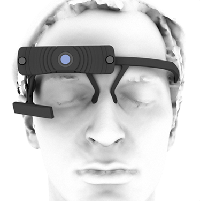
\includegraphics[scale=.7]{imagens/pupil.png}
\caption[]{Um rastreador de olhar acoplado à cabeça. Reproduzido de \protect \small{\url{https://pupil-labs.com/blog/2014-01/new-pupil-pro-headset-capture-software-0-3-7/}} }
\label{fig:pupil}
\end{center}
\end{figure}
%\footnotetext{\url{https://pupil-labs.com/blog/2014-01/new-pupil-pro-headset-capture-software-0-3-7/}}
}

Uma vantagem do rastreamento \textit{head-mounted} é que a câmera se move com a cabeça, então mudanças de pose não causam mudanças da posição da pupila na imagem. A desvantagem é a necessidade de usar um equipamento acoplado à cabeça. Por estar muito próxima do olho, a câmera do olho pode ocultar parte do campo de visão, dificultando a interação com o usuário.

\section{Características \newc{relevantes}}

Em algumas aplicações de rastreamento de olhar não estamos interessados apenas na direção do olhar em determinado instante, mas também podemos querer observar outras características relacionadas ao movimento do olhos. As características mais \oldc{específicas}\newc{relevantes} são \cite{lupung}:

\begin{itemize}
\item {\bf Fixação e sacada:} Em \newc{1879}, Emile Java (oftalmologista francês) observou que os movimentos do olho não ocorrem de forma contínua, e sim de movimentos rápidos, chamados de sacadas, seguidos por breves pausas, conhecidas como fixações \cite{lupung};

\item {\bf Área de interesse:} Região no ambiente que está presente no campo visual e que é de interesse em determinada pesquisa;

\item {\bf Duração do olhar:} Duração de um intervalo de tempo em que uma série de fixações está dentro de uma área de interesse;

\item {\bf Caminho de varredura:} localização espacial de uma sequência de fixações.
\end{itemize}
\chapter{\textit{Compressive Sensing}}

\textit{Compressive Sensing}(CS), também conhecido como \textit{Compressive Sampling} ou \textit{Compressed Sensing},  estuda formas de reconstruir um vetor a partir de poucas amostras. De agora em diante, será assumido que as amostras $(y_i)_{i = 1}^m$, representadas pelo vetor $y \in \mathbb{R}^m$ de um sinal $x \in \mathbb{R}^n$ são obtidas a partir de uma transformação linear $y = Ax$, onde $A$ é uma matriz $n \times m$, com $n < m$.

Como $n < m$, a equação não possui uma única solução $x$, se possuir. A idéia é então escolher, entre todas as soluções possíveis, o vetor $x$ com o maior número de coeficientes nulos. Para entender melhor o problema, as seguintes definições serão enunciadas:

\textbf{Def:} Seja $x \in \mathbb{R}^n$. $x$ é $k$-esparso se possui, no mínimo, $k$ coeficientes nulos.

\textbf{Def:} Dado $x \in \mathbb{R}^n$, a `norma' $0$ de $x$ é definida como
$\Vert x \Vert_{0} = \# \lbrace i : \vert x_i \vert > 0 \rbrace$ 

Observe que a `norma' 0 não é uma norma, pois, se $x = (1, 0)$, $\Vert 2x \Vert = 1 \neq 2 \Vert x \Vert$.

O problema será formulado da seguinte forma:

\begin{equation}
\tag{$P_0$}
\min_{x \in \mathbb{R}^n} \Vert x \Vert_{0} \textit{ sujeito a } Ax = y
\label{eqn:P0}
\end{equation}

No entanto, $\eqref{eqn:P0}$ é NP-difícil \cite{fourau}. Então tentamos resolver o seguinte problema:

\begin{equation}
\tag{$P_1$}
\min_{x \in \mathbb{R}^n} \Vert x \Vert_{1} \textit{ sujeito a } Ax = y
\label{eqn:P1}
\end{equation}

Um dos objetivos de CS é estudar condições para garantir a equivalência entre os dois problemas, e condições para a unicidade de soluções de $\eqref{eqn:P0}$ e $\eqref{eqn:P1}$. Para isso, essas condições foram estudadas.%Portanto, nesse período o aluno estudou essas condições.

%\section{Atividades realizadas}
%\subsection{Condições para equivalência entre $\eqref{eqn:P0}$ e $\eqref{eqn:P1}$}

%Durante esse período, o aluno pesquisou a teoria de Compressive Sensing (CS). Estudou e escreveu a demonstração de alguns dos principais teoremas, que fornecem:

%%\begin{itemize}

%\item Condições para garantir a unicidade de soluções do problema $\eqref{eqn:P0}$
%\begin{equation}
%\tag{$P_0$}
%\min_{x \in \mathbb{R}^n} \Vert x \Vert_{0} \textit{ sujeito a } Ax = y
%\label{eqn:P0}
%\end{equation}

%\item Condições para garantir a unicidade de soluções de $\eqref{eqn:P1}$
%\begin{equation}
%\tag{$P_1$}
%\min_{x \in \mathbb{R}^n} \Vert x \Vert_{1} \textit{ sujeito a } Ax = y
%\label{eqn:P1}
%\end{equation}

%\item Condições suficientes para a equivalência entre $\eqref{eqn:P0}$ e $\eqref{eqn:P1}$
%\end{itemize}

%CS tem como objetivo reconstruir um vetor $x \in \mathbb{R}^n$ a partir de poucas amostras. Assumindo que $x$ é esparso, podemos construir uma matriz $A$ de ordem $m \times n$, tal que $y = Ax$. A partir da amostra $y$, queremos recuperar o vetor $x$ resolvendo o problema $\eqref{eqn:P0}$, ou seja, queremos encontrar o vetor $x$ mais esparso com $y = Ax$.

%Fixado $k \in \{1, \hdots, n \}$, dizemos que $x$ é $k$-esparso se possui, no máximo, $k$ coeficientes não nulos. Seria interessante se cada amostra $y = Ax$ tivesse um único vetor $z$ $k$-esparso com $y = Az$. Nesse caso, a solução de $\eqref{eqn:P0}$ seria única.

\subsection{Unicidade de $\eqref{eqn:P0}$}
Se a matriz $A$ fosse $n \times n$ de posto máximo, a unicidade estaria garantida. Como $m < n$, definimos o conceito de \textit{spark}, que verbalmente é uma fusão dos conceitos `esparso' e `posto'(rank) \cite{kutyniok}.

\begin{definicao}
Seja $A$ uma matriz $m \times n$. O spark de $A$ denotado por $\textit{spark}(A)$ é o menor número de colunas linearmente dependentes de $A$.
\end{definicao}

O Teorema a seguir nos indica uma condição que $A$ deve satisfazer para garantir a unicidade de $\eqref{eqn:P0}$

\begin{teorema}
\label{thm:unicidade_P0}
Seja $A$ uma matriz $m \times n$. São equivalentes:

\begin{enumerate}[(i)]
\item $\textit{spark}(A)> 2k$

\item Para todo $y \in \mathbb{R}^m$, existe no máximo um $x \in \Sigma_k$ tal que $y = Ax$.
\end{enumerate}
\end{teorema}

Portanto, é desejável que $\textit{spark}(A)$ seja alto pois, nesse caso, seria possível recuperar vetores $x$ não tão esparsos.

Antes de demonstrar o teorema, enunciaremos uma definição e demonstraremos um lema.

\begin{definicao}
Dado $k \in \lbrace 1, \hdots , n \rbrace$,
$ \Sigma_k = \lbrace x : \Vert x \Vert_{0} \leq k \rbrace
           = \lbrace x : x $ é $k$-esparso$ \rbrace$
\end{definicao}

\begin{lema}
Dados $u, v \in \Sigma_k, u - v \in \Sigma_{2k}$
\end{lema}
\begin{proof}
Sejam $u, v \in \Sigma_k$. Então
\begin{subequations}
\begin{align*}
\Vert u - v \Vert_0 & \leq \Vert u \Vert_0 + \Vert -v \Vert_0 \\
& = \Vert u \Vert_0 + \Vert v \Vert_0 \\
& \leq k + k = 2k \\
& \Rightarrow u - v \in \Sigma_{2k}
\end{align*}
\end{subequations}
\end{proof}

Agora iremos demonstrar o Teorema \ref{thm:unicidade_P0}.
\begin{proof}
Seja $A$ uma matriz $m \times n$. Denote cada coluna $j$ de $A$ por $A_j$.
\begin{itemize}
\item $\neg$(i) $\Rightarrow$ $\neg$(ii)

Suponha que $\textit{spark}(A) \leq 2k$. Então existe um conjunto $J$ tal que $\#J = 2k$ e existe uma bijeção $\mu$ entre $\lbrace 1, \hdots, 2k \rbrace$ tais que

$$ \lbrace A_{\mu(j)} : j \in \lbrace 1, \hdots, 2k \rbrace \rbrace \text{ é LD }$$

Então existe $c \in R^{2k}, c \neq 0$ tal que

$$ \sum_{j = 1}^{2k} c_j A_{\mu(j)} = 0$$

Defina $u, v \in \mathbb{R}^n$ tais que, para $j \in \lbrace 1, \hdots, n \rbrace$

$$u_j = c_{\mu^{-1}(j)} \text{ se } j \in \mu^{-1}(\lbrace 1, \hdots, k \rbrace), 0 \text{ caso contrário}$$
$$v_j = -c_{\mu^{-1}(j)} \text{ se } j \in \mu^{-1}(\lbrace k+1, \hdots, 2k \rbrace), 0 \text{ caso contrário}$$

Se $j \in \mu^{-1}(\lbrace 1, \hdots, 2k \rbrace), u_j - v_j = c_j$. Então $u \neq v$\\
Então $\Vert u \Vert_0, \Vert v \Vert_0 \leq k \Rightarrow u, v \in \Sigma_k$.

Então
\begin{subequations}
\begin{align*}
\sum_{j = 1}^{2k} c_j A_{\mu(j)} &= \sum_{j = 1}^{k} c_j A_{\mu(j)} + \sum_{j = k+1}^{2k} c_j A_{\mu(j)}\\
& = \sum_{j = 1}^{k} u_{\mu(j)} A_{\mu(j)} - \sum_{j = k+1}^{2k} v_{\mu(j)} A_{\mu(j)} \\
& = Au - Av = 0 \\
 \Rightarrow Au = Av
\end{align*}
\end{subequations}

Então, definindo $y = Au$, existem $u, v \in \mathbb{R}^n$ distintos tais que $Au = Av$.
\item $\neg$(ii) $\Rightarrow$ $\neg$(i)

Suponha que existam $y \in \mathbb{R}^m$, $z, w \in \Sigma_k$ distintos tais que $y = Az = Aw$.

Seja $x = z - w$. Então $Ax = 0$ e, pelo lema anterior[sic], $x \in \Sigma_{2k}$. Além disso, $x \neq 0$.

Defina $K = \lbrace i \in \lbrace 1, \hdots, n \rbrace: \vert x_i \vert > 0 \rbrace$ e $\mu$ uma bijeção entre $\lbrace 1, \hdots, \Vert x \Vert_0 \rbrace$ e $K$. Então

$$ Ax = \sum_{j = 1}^{\Vert x \Vert_0} A_{\mu(j)} x_{\mu(j)} = 0$$

Como $x \neq 0$, existe algum $j \in \lbrace 1, \hdots, \Vert x \Vert_0 \rbrace$ tal que $x_{\mu(j)} \neq 0$. Logo, $A$ possui $\Vert x \Vert_0$ colunas linearmente dependentes. Portanto, $\textit{spark}(A) \leq \Vert x \Vert_0 \leq 2k$.
\end{itemize}
\end{proof}
\subsection{Unicidade de $\eqref{eqn:P1}$}

Ao encontrar a solução única de $\eqref{eqn:P0}$, encontramos o vetor desejado. No entanto, $\eqref{eqn:P0}$ é NP-difícil. Uma alternativa seria resolver o problema $\eqref{eqn:P1}$.

Precisamos então estudar a unicidade de soluções para $\eqref{eqn:P1}$ e condições para a equivalência entre $\eqref{eqn:P0}$ e $\eqref{eqn:P1}$, ou seja, em quais situações um vetor $x$ é solução única de ambos $\eqref{eqn:P0}$ e $\eqref{eqn:P1}$.

Definimos o conceito de \textit{Null space property} para estudar a unicidade de $\eqref{eqn:P1}$.

\begin{definicao} Seja $\Lambda \subset \lbrace 1, 2, \hdots, n \rbrace$. Defina $\Lambda^{\mathsf{c}} = \subset \lbrace 1, 2, \hdots, n \rbrace \setminus \Lambda$. Dado $x \in \mathbb{R}^n, x_{\Lambda} \in \mathbb{R}^n$, onde, para i $\in [n] = \{1, \hdots, n\}$

$$(x_{\Lambda})_i = 
\begin{cases}
x_i, &\mbox{se } i \in \Lambda \\
0,   &\mbox{caso contrário}
\end{cases}$$

\end{definicao}

\begin{definicao} Uma matriz A de tamanho $m \times n$ satisfaz a \textit{null space property}(NSP) relativa ao conjunto $\Lambda \subset [n]$ se para todo $h \in \ker(A) \setminus \lbrace 0 \rbrace$
%de ordem $k$ se existir uma constante $C > 0$ tal que

%para todo $h \in \ker(A), \Lambda \subset \lbrace 1, \hdots, n \rbrace \text{ tal que } \vert \Lambda \vert \leq k,$
%$$ \Vert h_{\Lambda} \Vert_2 \leq \frac{C \Vert h_{\Lambda^{\mathsf{c}}} \Vert_1}{\sqrt{k}} $$

%Estou usando a definicao do livro
$$ \Vert h_{\Lambda} \Vert_1 <  \Vert h_{\Lambda^{\mathsf{c}}} \Vert_1$$
\end{definicao}

\begin{definicao}
Dizemos que uma matriz de tamanho $m \times n$ satisfaz a \textit{null space property}(NSP) de ordem $k$ se ela satisfaz a NSP para todo $\Lambda \subset [n]$ com $\# \Lambda \leq k$.
\end{definicao}

\begin{lema}
Seja $\Lambda \in [n]$. Dado $x \in \mathbb{R}^n,$

$$ \Vert x \Vert_1 = \Vert x_{\Lambda} \Vert_1 + \Vert x_{\Lambda^{\mathsf{c}}} \Vert_1 $$
\end{lema}
\begin{proof} %Follow your nose.
$$
\Vert x \Vert_1 = \sum_{j = 1}^n \vert x_j \vert
= \sum_{j \in \Lambda}^n \vert x_j \vert + \sum_{j \in \Lambda^{\mathsf{c}}}^n \vert x_j \vert
= \Vert x_{\Lambda} \Vert_1 + \Vert x_{\Lambda^{\mathsf{c}}} \Vert_1
$$
\end{proof}

\begin{teorema}
Seja $A$ uma matrix $m \times n$. Todo vetor $x$ de suporte $\Lambda$ tal que $Ax = y$ é solução única de $\eqref{eqn:P1}$ se e somente se $A$ satisfaz a NSP para $\Lambda$.
\end{teorema}
\begin{proof}
Seja $A$ uma matrix $m \times n$.
\begin{itemize}

\item $( \Rightarrow )$

Seja $h \in \ker(A) \setminus \lbrace 0 \rbrace$. Então

$$ 0 = Ah = Ah_{\Lambda} + Ah_{\Lambda^{\mathsf{c}}} \Rightarrow Ah_{\Lambda} = - Ah_{\Lambda^{\mathsf{c}}} = A( -h_{\Lambda^{\mathsf{c}}} )$$

$h_{\Lambda}$ é solução única de $\eqref{eqn:P1}$, pois tem suporte $\Lambda$. Como $Ah_{\Lambda} = A( -h_{\Lambda^{\mathsf{c}}} )$, temos que

$$ \Vert h_{\Lambda} \Vert_1 < \Vert - h_{\Lambda^{\mathsf{c}}} \Vert_1
= \Vert h_{\Lambda^{\mathsf{c}}} \Vert_1 $$

Portanto $A$ satisfaz NSP para $\Lambda$.

\item $( \Leftarrow )$

Seja $x$ uma solução de $\eqref{eqn:P1}$ com suporte $\Lambda$ e $z \in \mathbb{R}^n$ tal que $Ax = Az$ e $z \neq x$. , Então $x - z \in \ker(A) \setminus \lbrace 0 \rbrace$. Definindo $w = \frac{z}{3}$, temos que

\begin{subequations}
\begin{align*}
\Vert x \Vert_1
& \leq \Vert x - w \Vert_1 + \Vert w \Vert_1 \\
& =    \Vert x_{\Lambda} - w_{\Lambda} \Vert_1
	 + \Vert x_{\Lambda^{\mathsf{c}}} - w_{\Lambda^{\mathsf{c}}} \Vert_1
	 + \Vert w \Vert_1 \\
& =    \Vert x_{\Lambda} - w_{\Lambda} \Vert_1
	 + \Vert w_{\Lambda^{\mathsf{c}}} \Vert_1
	 + \Vert w \Vert_1 \\
& <    \Vert x_{\Lambda^{\mathsf{c}}} - w_{\Lambda^{\mathsf{c}}} \Vert_1
	 + \Vert w_{\Lambda^{\mathsf{c}}} \Vert_1
	 + \Vert w \Vert_1 \\
& =    \Vert w_{\Lambda^{\mathsf{c}}} \Vert_1
	 + \Vert w_{\Lambda^{\mathsf{c}}} \Vert_1
	 + \Vert w \Vert_1 \\
& = 2 \Vert w_{\Lambda^{\mathsf{c}}} \Vert_1 + \Vert w \Vert_1 \\
& \leq 2 \Vert w \Vert_1 + \Vert w \Vert_1 \\
& = 3 \Vert w \Vert_1 = \Vert z \Vert_1
\end{align*}
\end{subequations}
Portanto $x$ é solução única de $\eqref{eqn:P1}$.
\end{itemize}
\end{proof}


A noção de NSP nos diz que a norma 1 dos vetores do núcleo de $A$ não estão concentradas num número pequeno de índices. O Corolário \ref{cor:unicidade_P1} estabelece uma relação entre NSP e a unicidade de soluções de $\eqref{eqn:P1}$.

\begin{corolario}
\label{cor:unicidade_P1}
Seja $A$ uma matrix $m \times n$. Todo vetor $x$ $k$-sparso tal que $Ax = y$ é solução única de $\eqref{eqn:P1}$ se e somente se $A$ satisfaz a NSP de ordem $k$.
\end{corolario}
\begin{proof}
Seja $A$ uma matrix $m \times n$.
\begin{itemize}

\item $( \Rightarrow )$

Seja $\Lambda \subset [n]$ tal que $\# \Lambda = k$. Seja $x$ um vetor esparso de suporte em $\Lambda$ tal que $x$ é solução única de $\eqref{eqn:P1}$. Então, [pelo teorema anterior], $A$ satisfaz NSP para $\Lambda$. Como $\Lambda$ é arbitrário, $A$ satisfaz NSP de ordem $k$.

\item $( \Leftarrow )$

Seja $x$ um vetor $k$-esparso tal que $Ax = y$. Então existe $\Lambda \subset [n]$ tal que $\# \Lambda = k$ e $x_{\Lambda} = x$. Como $A$ satisfaz NSP para $\Lambda$, $x$ é solução única.
\end{itemize}
\end{proof}

\subsection{Equivalência entre $\eqref{eqn:P0}$ e $\eqref{eqn:P1}$}
Para estudar a equivalência entre $\eqref{eqn:P0}$ e $\eqref{eqn:P1}$, por enquanto, assumimos que as colunas $a_i$ de $A$ possuem norma $\Vert a_i \Vert_2 = 1$. Definimos também o conceito de coerência.

\begin{definicao}
Seja $A$ uma matriz $m \times n$ cujas colunas $a_i$ possem $\Vert a_i \Vert_2 = 1$. definimos a coerência (ou \textit{mutual coherence}) de $A$, denotada por $\mu(A)$, como

%$$\mu(A) = \max_{i \neq j} \frac{\vert \langle a_i, a_j \rangle \vert}{\Vert a_i \Vert_2 \Vert a_j \Vert_2} $$

$$\mu(A) = \max_{i \neq j} \vert \langle a_i, a_j \rangle \vert$$
\end{definicao}

O seguinte teorema, que garante a equivalência entre $\eqref{eqn:P0}$ e $\eqref{eqn:P1}$ foi então estudado.

\begin{teorema}
Seja $x$ uma solução de $\eqref{eqn:P0}$ tal que

$$ \Vert x \Vert_0 < \frac{1}{2} \left(1 + \frac{1}{\mu(A)}\right) $$

Então $x$ é solução única de $\eqref{eqn:P0}$ e $\eqref{eqn:P1}$.
\label{thm:equivalencia_P0P1}
\end{teorema}

Alguns resultados serão apresentados antes de demonstrar o Teorema \ref{thm:equivalencia_P0P1}.

\begin{definicao}
Seja $x \in \mathbb{R}^n$. Definimos $\vert x \vert$ como um vetor $\vert x \vert \in \mathbb{R}^n$ tal que para cada $i \in [n], \vert x \vert_i = \vert x_i \vert$.
\end{definicao}

\begin{definicao}
Dados $x, y \in \mathbb{R}^n, x \leq y$ se $\forall j \in [n], x_i \leq y_i$.
\end{definicao}

\begin{lema}
Fixado $x \in \mathbb{R}^n, x \leq \vert x \vert$.
\end{lema}
\begin{proof}
$ \forall i \in [n], x_i \leq \vert x_i \vert = \vert x \vert_i$
\end{proof}

\begin{lema} %fazer alguma observacao para ficar mais claro
Dado $x \in \mathbb{R}^n, \Vert x \Vert_1 = \Vert \vert x \vert \Vert_1$
\end{lema}
\begin{proof}
Seja $x \in \mathbb{R}^n$,

$$\Vert x \Vert_1 = \sum_{i = 1}^n \vert x_i \vert = \sum_{i = 1}^n \vert (\vert x_i \vert) \vert
= \sum_{i = 1}^n \vert (\vert x \vert_i) \vert = \Vert \vert x \vert \Vert_1$$
\end{proof}

\begin{definicao}
Seja $A$ uma matriz $m \times n$. $\vert A \vert$ é uma matriz $m \times n$ cujas entradas $\vert A \vert_{ij} = \vert A_{ij} \vert$, para todo $i \in [m], j \in [n]$.
\end{definicao}

\begin{lema}
Sejam $A$ uma matriz $m \times n$ e $x \in \mathbb{R}^n$. Então $\vert Ax \vert \leq \vert A \vert \vert x \vert$.
\end{lema}
\begin{proof}
Dado $i \in [n]$,

$$ \vert Ax \vert_i = \vert (Ax)_i \vert = \left| \sum_{k = 1}^n A_{ik}x_k \right|
\leq  \sum_{k = 1}^n \vert A_{ik}x_k \vert 
=     \sum_{k = 1}^n \vert A_{ik} \vert \vert x_k \vert
=     (\vert A \vert \vert x \vert)_i
$$
\end{proof}

\begin{teorema}
(citar referência) Seja $A$ uma matriz $n \times n$, de elementos $a_{ij}, 1\leq i,j \leq n$. Então, para cada autovalor $\lambda$ de $A$,

$$ \lambda \in \bigcup_{i = 1}^n \overline{B}(a_{ii}, r_i) $$

onde $$r_i = \sum_{j \neq i} \vert a_{ij} \vert$$
\end{teorema}
\begin{proof}
Sejam $\lambda \in \mathbb{C}$ um autovalor de $A$, $v \in \mathbb{C}^{n}$ tal que $Av = \lambda v$. Escolha $i \in [n]$ de forma que $\vert v_j \vert \leq \vert v_i \vert$, para todo $j \in [n]$. Então $v_i \neq 0$ e

\begin{subequations}
\begin{align*}
& \lambda v_i = (Av)_i
= \sum_{j = 1}^n a_{ij}v_j
= a_{ii}v_i + \sum_{j \neq i} a_{ij}v_j
\\ \Rightarrow &
(\lambda - a_{ii})v_i = \sum_{j \neq i} a_{ij}v_j
\\ \Rightarrow &
\vert \lambda - a_{ii} \vert \vert v_i \vert \leq \sum_{j \neq i} \vert a_{ij} \vert \vert v_j \vert
\\ \Rightarrow &
\vert \lambda - a_{ii} \vert \leq
\sum_{j \neq i} \vert a_{ij} \vert \frac{ \vert v_j \vert}{\vert v_i \vert}
\leq \sum_{j \neq i} \vert a_{ij} \vert = r_i
\\ \Rightarrow &
\lambda \in \overline{B}(a_{ii}, r_i)
\end{align*}
\end{subequations}
\end{proof}

\begin{lema}
Para toda matriz real $A$ de tamanho $m \times n$, com colunas $a_i$ tais que $\Vert a_i \Vert_2 = 1,$
$$spark(A) \geq 1 + \frac{1}{\mu(A)}$$
\end{lema}
\begin{proof}
Seja $G = A^{\mathsf{T}}A$. Para todo  $i \in [m], G_{ii} = 1$. Para $i \neq j$, $G_{ij} = \langle a_i, a_j \rangle \leq \Vert a_i \Vert_2 \Vert a_j \Vert_2 = 1$. Logo, $\mu(A) \leq 1$. Então, para todo $\lambda$ autovalor de $G$,

$$ \vert \lambda - 1 \vert \leq \sum_{j \neq i} \vert G_{ij} \vert \leq (m - 1)$$

% $G$ é real e simétrica, então todos seus autovalores são positivos. 
\end{proof}
%\section{Atividades realizadas}

%Durante o período, o aluno estudou um algoritmo para resolver $\eqref{eqn:P1}$ e estudou técnicas de rastreamento de olhar.

%\subsection{Minimização de norma 1}

Agora demonstraremos o Teorema \ref{thm:equivalencia_P0P1}.
\begin{proof}

[CORRIGIR: Assumindo que x é solução única de $\eqref{eqn:P0}$]

[ESCREVER LEMA $\vert v + m\vert - \vert v \vert \geq -\vert m \vert$]

Seja $z \in \mathbb{R}^n$ tal que $z \neq x$. Então $z = x + h$ para algum $h \in \ker(A) \setminus{0}$.
Seja $\Lambda$ o suporte de $x$. Temos que

\begin{subequations}
\begin{align*}
\Vert z \Vert_1 - \Vert x \Vert_1 &
= \sum_{k = 1}^n \vert x_k + h_k \vert - \sum_{k = 1}^n \vert x_k \vert \\
& = \sum_{k \in \Lambda} \vert x_k + h_k \vert +
\sum_{k \in \Lambda^{\mathsf{c}}} \vert x_k + h_k \vert
- \sum_{k \in \Lambda} \vert x_k \vert \\
& = \sum_{k \in \Lambda} \vert x_k + h_k \vert +
\sum_{k \in \Lambda^{\mathsf{c}}} \vert h_k \vert
- \sum_{k \in \Lambda} \vert x_k \vert \\
& = \sum_{k \in \Lambda^{\mathsf{c}}} \vert h_k \vert
+ \sum_{k \in \Lambda} \left( \vert x_k + h_k \vert - \vert x_k \vert \right) \\
& \geq \sum_{k \in \Lambda^{\mathsf{c}}} \vert h_k \vert
- \sum_{k \in \Lambda} \vert h_k \vert \\
& = \Vert h_{\Lambda^{\mathsf{c}}} \Vert_1 - \Vert h_\Lambda \Vert_1
\end{align*}
\end{subequations}

Pelo [LEMA ...],
$$\inf_{\substack{Ah = 0 \\ h \neq 0}} \Vert h \Vert_1 - 2 \Vert h_\Lambda \Vert_1
= \inf_{\substack{Ah = 0 \\ \Vert h \Vert_1 = 1}} \Vert h \Vert_1 - 2 \Vert h_\Lambda \Vert_1
= \inf_{\substack{Ah = 0 \\ \Vert h \Vert_1 = 1}} 1 - 2 \Vert h_\Lambda \Vert_1
$$

Como $Ah = 0 \Rightarrow A^{\mathsf{T}} A h = 0$, temos que

$$ \inf_{\substack{Ah = 0 \\ \Vert h \Vert_1 = 1}} 1 - 2 \Vert h_\Lambda \Vert_1
\geq \inf_{\substack{A^{\mathsf{T}}Ah = 0 \\ \Vert h \Vert_1 = 1}} 1 - 2 \Vert h_\Lambda \Vert_1$$

Como $ \Vert h \Vert_1 = \Vert \vert h \vert \Vert_1$ e $\vert h_\Lambda \vert = \vert h \vert_\Lambda$, temos que

$$\inf_{\substack{A^{\mathsf{T}}Ah = 0 \\ \Vert h \Vert_1 = 1}} 1 - 2 \Vert h_\Lambda \Vert_1
\geq \inf_{\substack{A^{\mathsf{T}}Az = 0 \\ \Vert z \Vert_1 = 1 \\ z \geq 0}}
1 - 2 \Vert z_\Lambda \Vert_1$$

Definindo $G = A^{\mathsf{T}}A$, cada entrada $G_{ij} = \langle a_i, a_j \rangle$.
%Como $Gz = 0$, $Gz - z = -z \Rightarrow (G - I)z = -z$. Então
%[provar que $\vert \alpha z \vert = \vert \alpha \vert \vert z \vert$]

$$\inf_{\substack{A^{\mathsf{T}}Az = 0 \\ \Vert z \Vert_1 = 1 \\ z \geq 0}}
1 - 2 \Vert z_\Lambda \Vert_1
=
\inf_{\substack{Gz = 0 \\ \Vert z \Vert_1 = 1 \\ z \geq 0}}
1 - 2 \Vert z_\Lambda \Vert_1$$

Como $z \geq 0$ e $Gz = 0$,
$$ z = \vert -z \vert \Rightarrow z = \vert Gz - z \vert
= \vert (G - I)z \vert \leq \vert G - I \vert z
$$

Todos as entradas de $G - I$ maiores os iguais a zero e os elementos da diagonal são nulos, então
$$ \vert G - I \vert_{ij} \leq \max_{i \neq j} G_{ij} = \max_{i \neq j} \langle a_i, a_j \rangle = \mu(A)$$
Então
$$ \vert G - I \vert \leq \mu(A) (\mathbb{1} - I)$$

Logo
$$ z \leq \mu(A) (\mathbb{1} - I) z$$

Então, dado $i \in \Lambda$,

\begin{subequations}
\begin{align*}
z_i & \leq \mu(A) \left( \sum_{j = 1}^n z_j - z_i \right) \\
& \leq \mu(A) (\Vert z \Vert_1  - z_i) \\
& = \mu(A)(1 - z_i) \\
\Rightarrow z_i + z_i\mu & \leq \mu(A)\\
\Rightarrow z_i &\leq \frac{\mu(A)}{1 + \mu(A)}
\end{align*}
\end{subequations}

Então

$$ \Vert z_\Lambda \Vert_1
= \sum_{i \in \Lambda} z_i
\leq \sum_{i \in \Lambda} \frac{\mu(A)}{1 + \mu(A)}
= \Vert x \Vert_0 \frac{\mu(A)}{1 + \mu(A)}
$$

Então

\begin{subequations}
\begin{align*}
\inf_{\substack{Gz = 0 \\ \Vert z \Vert_1 = 1 \\ z \geq 0}}
1 - 2 \Vert z_\Lambda \Vert_1
& \geq
\inf_{\substack{Gz = 0 \\ \Vert z \Vert_1 = 1 \\ z \geq 0}}
1 - 2 \Vert x \Vert_0 \frac{\mu(A)}{1 + \mu(A)} \\
& >
\inf_{\substack{Gz = 0 \\ \Vert z \Vert_1 = 1 \\ z \geq 0}}
1 - 2 \frac{1}{2} \left(1 + \frac{1}{\mu(A)}\right) \frac{\mu(A)}{1 + \mu(A)} \\
& = 1 - 2 \frac{1}{2} \left(1 + \frac{1}{\mu(A)}\right) \frac{\mu(A)}{1 + \mu(A)} \\
& = 1 - \frac{\mu(A) + 1}{\mu(A)} \frac{\mu(A)}{1 + \mu(A)}\\
& = 1 - 1 = 0
\end{align*}
\end{subequations}
\end{proof}

\section{Matrizes que satisfazem as condições de CS}

Como vimos anteriormente, a matriz $A$ deve satisfazer algumas condições para garantir a equivência entre $\eqref{eqn:P0}$ e $\eqref{eqn:P1}$, que chamaremos que condições de CS. Em vez de construir uma matriz $A$ de forma determinística, o que talvez não seja fácil, podemos construir uma matriz aleatória que satisfaz as condições de CS.

%A seguir, listaremos algumas matrizes que satisfazem essas condições com alta probabilidade.

%http://www.math.ucla.edu/~wotaoyin/summer2013/slides/Lec03_SparseRecoveryGuarantees.pdf

Uma matriz $A$ cujas entradas são amostradas através de uma distribuição normal satisfazem as condições de CS com alta probabilidade, como mostra o Teorema \ref{thm:normalCS}.

\begin{teorema} \cite{zhang2008theory} Sejam $m < n$, $\Omega \subset \mathbb{R}^n$ e $A \in \mathbb{R}^{m \times n}$ tais que apenas uma das afirmações é verdadeira:
\begin{enumerate}
\item os elementos $a_ij$ de A são iid e $a_{ij} \sim \mathcal{N}(0,1)$
\item $A$ é uma matriz de posto $m$ com $BA^{\texttt{T}} = 0$ para uma matriz $B \in \mathbb{R}^{(n - m) \times n}$ cujas entradas são iid $\mathcal{N}(0,1)$.
\end{enumerate}
Então com probabilidade maior que $1 - e^{-c_0(n-m)}$, $\bar{x}$ é solução única de $\eqref{eqn:P0}$ e $\eqref{eqn:P1}$ se $\bar{x}$ satisfaz

$$ \Vert \bar{x} \Vert_0 < \frac{{c_1}^2}{4} \frac{m}{1 + \log(n/m)}$$

onde $c_0, c_1 > 0$ são constantes independentes das dimensões $m$ e $n$.
\label{thm:normalCS}
\end{teorema}
\chapter{O algoritmo de homotopia}

O algoritmo de Homotopia é um algoritmo com o objetivo de resolver $\eqref{eqn:P1}$ minimizando funções do tipo
$$J_{\lambda_n}(x) = \frac{1}{2} \Vert Ax - y \Vert_2^2 + \lambda_n \Vert x \Vert_1$$
para uma sequência decrescente $(\lambda_n)$ de números positivos.

Podemos encontrar o mínimo de uma função diferencial $f: \mathbb{R}^n \longrightarrow \mathbb{R}$ procurando os pontos $x$ no domínio em que $\nabla f(x) = 0$. No nosso caso, a norma $1$ não é diferenciável. Então será definida uma generalização para a diferencial, que será usada no algoritmo, chamado de Homotopia.

\begin{definicao}
Seja $f: \mathbb{R}^n \longrightarrow \mathbb{R}$. A subdiferencial de $f$ em $x \in \mathbb{R}$ é dada por

$$\partial f(x) = \{ v \in \mathbb{R}^N : f(y) - f(x) \geq \langle v, y - x \rangle, \forall y \in \mathbb{R}^N \}$$

%Mostrar que a subdiferencial é uma generalização da diferencial
% >>> http://www.staff.science.uu.nl/~balde101/cao10/cursus10_1.pdf
\end{definicao}

Não é difícil ver que o operador $\partial$ é linear. A subdiferencial coincide com a diferencial de uma função, quando ela for convexa e diferenciável, como mostra a seguinte proposição:

\begin{proposicao}
Se $f: \mathbb{R}^n \longrightarrow \mathbb{R}$ for convexa e diferenciável, então para todo $x \in \mathbb{R}^n$, $\partial f(x) = \{ \nabla f(x) \}$.
\end{proposicao}
%\begin{proof}
%Dados $x, y \in \mathbb{R}^n$, defina a seguinte curva $\gamma: \left[0,1\right]$.
%\end{proof}

Um ponto $x_0$ é ponto de mínimo de uma função $f$ se, e somente se, $0 \in \partial f$, pois
$$ \forall x \in \mathbb{R}^n, f(x) - f(x_0) \geq 0 = \langle 0, x - x_0 \rangle$$.

%Explicar melhor, por exemplo, dizer que \partial (v1, v2) = \partial v1 \times \partial v2
Como a norma $1$ é convexa, sua subdiferencial em um ponto $x$ é um vetor $v$ tal que para cada $i = 1, \hdots, n$,
$$ v_i =
\begin{cases}
	sgn(v_i) & \mbox{ se } v_i \neq 0 \\
	\lbrace 1, -1\rbrace & \mbox{ se } v_i = 0
\end{cases}$$
%Citar FornasireFinal_red.pdf, que definiu a subdiferencial de f

%@inproceedings{yang2010fast,
%  title={Fast ℓ 1-minimization algorithms and an application in robust face recognition: A review},
%  author={Yang, Allen Y and Sastry, S Shankar and Ganesh, Arvind and Ma, Yi},
%  booktitle={2010 IEEE International Conference on Image Processing},
%  pages={1849--1852},
%  year={2010},
%  organization={IEEE}
%}

O algoritmo de Homotopia \cite{fornasier} \cite{dontsa} minimiza a função em um número finito de passos. Fixado um $\lambda$ positivo, considere a seguinte função :

$$J_{\lambda} (x) = \frac{1}{2} \Vert Ax - y \Vert_2^2 + \lambda \Vert x \Vert_1$$

%citar quem mostra que a curva é linear por partes
e seu respectivo minimizador $x_\lambda$. Quando $\lambda$ é grande, $x_{\lambda} = 0$. O ponto $\tilde{x}$, solução de $\eqref{eqn:P1}$ é solução de algum $J_{\tilde{\lambda}}$. A curva $\lambda \longmapsto x_{\lambda}$ é linear por partes, então é possível encontrar a solução de $\eqref{eqn:P1}$ com um número finito de passos.

A subdiferencial de $J_\lambda$ é

$$\partial J_\lambda(x) = A^{T}(Ax - y) + \lambda \partial \Vert x \Vert_1$$

Se $x = x_\lambda$ então $0 \in \partial J_\lambda(x)$ é equivalente a

\begin{equation}
\begin{cases}
(A^*(Ax - y))_i           =    \lambda sgn(x_i), &\mbox{se } x_i = 0\\
\vert A^*(Ax - y)\vert_i  \leq \lambda,          &\mbox{se } x_i \neq 0
\end{cases}
\label{eqn:hom0}
\end{equation}

para $i \in \{1, \hdots, n \}$. Escrevendo $c = A^{T}(Ax - y)$ e denotando $I$ como o suporte de $x$, então $\eqref{eqn:hom0}$ equivale a

\begin{equation}
\begin{cases}
c(I)           =    \lambda sgn(x_{\lambda}(I)) \\
\vert c(I^{\texttt{c}}) \vert \leq \lambda
\end{cases}
\label{eqn:hom1}
\end{equation}

O algoritmo de Homotopia procura os vértices da curva $\lambda \longmapsto x_\lambda$. Começando com $x_0 = 0$, em uma iteração $l$, $\lambda_l = \Vert c(I) \Vert_{\infty}$, com $I$ denotando o suporte de $x_l$. Depois, o algoritmo calcula uma direção $d_l$, onde

\begin{equation}
\begin{cases}
A^{\texttt{T}}_I A_I d_l(I) = sgn (c_l(I)) \\
d_l(I^{\texttt{c}}) = 0
\end{cases}
\label{eqn:hom2}
\end{equation}

A magnitude $\gamma_l$ do passo $d_l$ é calculada como o menor valor em que a equação $\eqref{eqn:hom1}$ não seja mais válida, ou seja, para $x_{l+1} = x_{l} + \gamma_l d_l$, teremos que pelo menos uma das seguintes condições será satisfeita:

\begin{enumerate}[(i)]
\item para algum $i \in I, \vert (c_l)_i \vert \ > \lambda$. Isso ocorre para $\gamma_l = \gamma_l^{+}$, onde
$$ \gamma_l^{+} = \min_{i \in I^c} \left\lbrace \frac{\lambda_l - c_l(i)}{1 - a_i^T v_l}, \frac{\lambda_l + c_l(i)}{1 + a_i^T v_l} \right\rbrace$$

\item para algum $i \in I, (x_{l+1})_i = 0$, o que equivale a $\gamma = \gamma^{-}$, onde
$$ \gamma_l^{-} = \min_{i \in I} \left\lbrace \frac{- x_l(i)}{d_l(i)} \right\rbrace$$
\end{enumerate}

Então calculamos $\gamma = \min \lbrace \gamma_l^{-}, \gamma_l^{+} \rbrace$. O algoritmo termina quando $c_l = 0$.
\chapter{O modelo \textit{cross-and-bouquet}}

%O modelo \textit{cross-and-bouquet} usa CS para classificar imagens, no caso, dado um $frame$ encontrar a imagem em um dicionário mais parecida ele.

O modelo \textit{cross-and-bouquet} usa \oldc{CS}\textit{Compressive Sensing} para classificar imagens, ou seja, dada uma amostra $y$ e uma família de imagens \oldc{$(\Phi_i)$}\newc{$(a_i)_{i=1}^n$}, encontrar qual \oldc{$\Phi_i$}\newc{$a_i$} é mais \oldc{próxima}\newc{próximo} de $y$.

Podemos interpretar o problema $\eqref{eqn:P0}$ da seguinte forma: dado um vetor $y \in \mathbb{R}^m$, quais colunas $a_i \in \mathbb{R}^m$ de $A$ melhor representam $y$? Se $y$ puder ser escrito como $y = Ax$ com $x$ esparso, podemos assumir que a coluna $a_i$ mais próxima de $y$ é aquela onde $x_i$ possui maior valor absoluto, ou seja,

$$ i = \argmax_{j = 1, \hdots, n} \vert x_j \vert $$

%Dado um conjunto de sinais $a_i \in \mathbb{R}^m$ com $A = \left[ a_1 \vert \hdots \vert a_m]$ e uma amostra $y \in \mathbb{R}^m$
Como vimos, CS garante que conseguimos encontrar $x$ esparso resolvendo $\eqref{eqn:P1}$ apenas quando $A$ é incoerente. Em aplicações, como em processamento de imagens, os vetores $a_i$ não são ``muito diferentes'' entre si, por isso não podemos assumir que $A$ é incorente. Então formularemos o problema de uma forma um pouco diferente:

Dado $y \in \mathbb{R}^m$ e $A$ uma matriz $m \gg n$ (ou seja, o número de amostras é pequeno se comparado à dimensão de cada amostra),

\begin{equation}
\tag{$\tilde{P_1}$}
\min_{x \in \mathbb{R}^n} \Vert x \Vert_{1} + \Vert e \Vert_{1} \textit{ sujeito a } y = Ax + e
%\label{eqn:P1_tilde}
\end{equation}

o que é equivalente a encontrar um vetor $c = \left[ \begin{tabular}{c}
x \\
e
\end{tabular} \right]$, com $x \in \mathbb{R}^n$ e $e \in \mathbb{R}^m$, onde $c$ resolve o problema

\begin{equation}
\tag{$\tilde{P_1}$}
\min_{c \in \mathbb{R}^{n + m}} \Vert c \Vert_{1} \textit{ sujeito a } y = \left[ \begin{tabular}{c c} A &  I \end{tabular} \right] c
\label{eqn:P1_tilde}
\end{equation}

onde $I$ é a matriz identidade $m \times m$.

Como $I$ é incoerente, pois é ortonormal, e possui muito mais colunas que $A$, é razoável supor que $\left[\begin{tabular}{c c} A &  I \end{tabular} \right]$ também seja incoerente e, neste caso, a solução $c$ de $\eqref{eqn:P1_tilde}$ seria esparsa.

Identificamos a amostra $y$ com o vetor $a_i$ onde
$$i = \argmax_{i = 1, \hdots, n} \vert c_i \vert$$

Essa é a ideia do modelo \textit{cross-and-bouquet} \cite{wrima}. O modelo tem esse nome porque as colunas de $I$ são ortonormais, lembrando uma cruz e as colunas de $A$ estão próximas, lembrando um buquê, como mostra a Figura \ref{fig:cross_bouquet}.

\begin{figure}
\centering
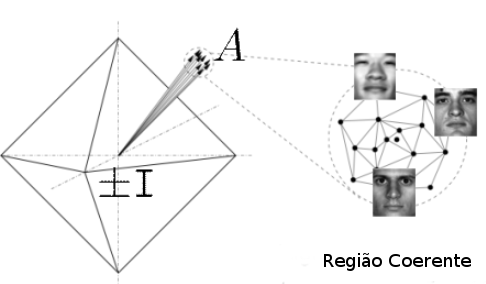
\includegraphics[scale=.6]{imagens/cross-and-bouquet.png}
\caption{Modelo \textit{cross-and-bouquet}. Imagem representando as colunas de $\left[ A \vert I \right]$ onde cada coluna de $A$ pode representar uma imagem, por exemplo. Adaptado de \cite{yangetal}.}
\label{fig:cross_bouquet}
\end{figure}

\section{Desempenho}

Dada uma imagem $y$, poderíamos ter identificado a imagem com a amostra $a_i$ que maximiza a correlação entre $a_i$ e $y$. Desenvolvemos um programa para classificar imagens do olho usando correlação e \textit{cross-and-bouquet}.

Coletamos imagens de uma pessoa olhando para pontos dispostos numa grade $7 \times 7$ no monitor, como descrito no Capítulo $6$.  Calculamos a matriz $A$ usando a primeira imagem registrada para cada amostra e selecionamos aleatoriamente $5$ imagens do olhos correspondendo a cada posição da grade. Para cada imagem $y$, estimamos a posição da grade correspondente a $y$ como:

\begin{itemize}
\item {\bf Correlação:} usando correlação, estimamos a posição cuja coluna $a_i$ apresenta maior correlação em módulo entre $a_i$ e $y$;

\item {\bf \textit{Cross-and-bouquet:}} identificamos a coluna $a_i$ mais próxima de $y$ usando o modelo \textit{cross-and-bouquet}.
\end{itemize}

Testamos para diferentes tamanhos de imagem e, calculamos a taxa de acertos (ou seja, a quantidade de vezes em que o algoritmo identificou a posição correta do olhar dividido pelo número de imagens usadas, $5 \times 7 \times 7 = 245$). A Tabela  $\ref{tab:acertos_cross}$ mostra os resultados para diferentes tamanhos de imagem. O melhor resultado calculado usando correlação é bem inferior aos resultados calculados usando \textit{Compressive Sensing}.

\begin{table}
\centering
\begin{tabular}{| c | c | c | c |}
\hline
{\bf proporções da imagem} & {\bf correlação} & {\bf \textit{cross-and-bouquet}}  \\ \hline
$640 \times 480$ & $14,29\%$	 & ---\\ \hline
$320 \times 240$ & $12,25\%$	 & ---\\ \hline
$160 \times 120$ & $10,20\%$	 & ---\\ \hline
$80 \times 60$   & $8,16\%$		 & $90,61\%$ \\ \hline
$40 \times 30$	 & $6,12\%$		 & $91,02\%$ \\ \hline
$20 \times 15$	 & $2,04\%$		 & $86,94\%$ \\ \hline
\end{tabular}
\caption{Desempenho dos algoritmos de correlação e \textit{cross-and-bouquet} para identificar imagens. Note que o desempenho é muito inferior quando usamos correlação.}
\label{tab:acertos_cross}
\end{table}
\chapter{Desenvolvimento de um rastreador de olhar usando CS}

\newc{Alguns algoritmos de rastreamento de olhar usam técnicas de processamento de imagens para identificar a posição da pupila. Essa tarefa é dificultada pela oclusão parcial da pupila pelos cílios. Em vez de estimar a posição da pupila, podemos comparar a imagem com amostras de imagens do olho onde a posição do olhar é conhecida e depois estimar o olhar a partir das posições de olhar das amostras mais parecidas com a imagem atual.

Usamos o modelo \textit{cross-and-bouquet} para comparar imagens das amostras e estimar a posição do olhar.}

Desenvolvemos um programa para estimar o olhar do usuário, ou seja, estimar qual coordenada $(x,y)$ na tela o usuário está olhando. Para isso, usamos câmera da Pupil Labs para coletar imagens do olho direito. Essa câmera fica acoplada à cabeça e registra imagens em infravermelho \footnote{\url{https://github.com/pupil-labs/pupil/wiki/Environment}}. O programa é dividido em duas etapas principais:

\begin{itemize}
\item {\bf Calibração:} exibimos alvos em posições específicas na tela e coletamos uma imagem do olho por alvo, assumindo que o usuário está olhando para o alvo.

\item {\bf Rastreamento:} para cada frame $f$, encontramos as amostras mais parecidas com $f$. Estimamos a posição do olhar como a média das posições da na tela correspondentes às amostras selecionadas.
\end{itemize}

Essas etapas são descritas mais detalhadamente abaixo.

\section{Coleta de amostras}

%Nesta etapa, o programa coleta uma imagem do olho correspondendo a cada uma das coordenadas na tela de uma grade com $10 \times 10$ pontos. Para cada alvo, é necessário que o usuário pressione uma tecla quando estiver olhando para o alvo para ler a amostra, como mostra a Figura \ref{fig:alvo}. Assumimos que o usuário não move a cabeça durante a coleta.

Fizemos o experimento com seis pessoas para avaliar o desempenho do rastreador de olhar. Durante o experimento o participante ficou sentado a $56,5cm$ de distância do monitor, com o olho direito alinhado com o centro da tela. Para evitar movimentos da cabeça durante a coleta das imagens, a pessoa ficou com o queixo apoiado sobre o punho e cotovelo correspondente apoiado na mesa. Registramos imagens do olho direito usando uma câmera do Pupil Labs, acoplada à cabeça, que grava imagens em infravermelho.

A câmera do Pupil Labs estava ligada a um suporte de formato parecido com uma armação de óculos. Por esse motivo, quem usa óculos teve que retirar os óculos para participar do experimento.

Antes de iniciar a coleta, mostramos a imagem da câmera do olho para a pessoa ajustar a câmera de forma que o olho inteiro esteja visível na imagem, como mostra a Figura \ref{fig:ajustando_olho}.

\begin{figure}
\centering
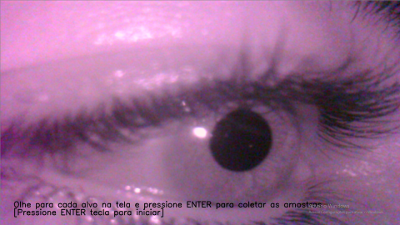
\includegraphics[scale=1]{imagens/ajustando_camera.png}
\caption{O programa exibe uma imagem do olho antes da coleta, para o usuário ajustar a câmera de forma que o olho inteiro seja registrado.}
\label{fig:ajustando_olho}
\end{figure}

Foram exibidos aleatoriamente $49$ pontos dispostos numa grade $7 \times 7$ de pontos igualmente espaçados, onde a distância entre cada lado da grade e o canto correspondente da tela corresponde a um grau do campo visual.

Mostramos cada alvo individualmente durante dois segundos e o usuário deveria olhar para o ponto, como mostra a Figura $\ref{fig:alvo}$. Mostramos os pontos aleatoriamente para evitar aprendizado do usuário, ou seja, evitar que o usuário olhe para o ponto correspondendo à amostra seguinte antes de terminar a coleta da amostra atual. Apesar de mostrar cada ponto durante dois segundos, coletamos imagens apenas após o primeiro segundo porque durante os primeiros instantes ocorre a sacada, ou seja, o movimento do olhar até a região de interesse, e queremos registrar apenas imagens correspondendo à fixação, ou seja, quando a pessoa está realmente olhando para o ponto.

%Coletamos um número grande (cerca de 25 amostras por usuário por posição da tela) de imagens porque queremos comparar o desempenho de programa usando diferentes números de amostras para calibrar o rastreador, como explicaremos adiante.
Usamos um monitor de lagura $37,3cm$ e altura de $32cm$, com resolução $1280 \times 1024$. A coleta durou menos de $10$ minutos por participante.

\begin{figure}
\centering

\includegraphics[scale=1]{imagens/alvo.png}
\caption{\oldc{Durante uma coleta, a pessoa deve olhar. Os alvos são exibidos em posições diferentes em uma grade $7 \times 7$ na tela.} \newc{Durante uma coleta, a pessoa deve olhar para os alvos que são exibidos em posições diferentes em uma grade $7 \times 7$.}}
\label{fig:alvo}
\end{figure}

\section{\newc{Rastreamento de olhar}}

Após terminar a coleta das imagens, estimamos a posição do olhar para imagens correspondendo a todos os pontos da grade $7 \times 7$. Como todas imagens registradas correspondem aos pontos da grade, já sabemos a posição do olhar em cada um deles, então usaremos a posição exata e a posição estimada para calcular o erro como a distância euclidiana entre elas. Usaremos a posição de cada alvo em graus horizontal e vertical, e não em \textit{pixels} na tela.

Para cada posição na grade, consideramos a primeira imagem coletada como a amostra correspondente àquela posição na tela, e estimaremos a posição do olhar para cinco das outras imagens, selecionadas aleatoriamente, comparando esta com todas as amostras\newc{, como mostra a Figura $\ref{fig:matriz_olho}$.}

\begin{figure}
$$ A = \left[ \hspace{2pt} \raisebox{-9pt}{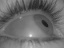
\includegraphics[scale=.6]{imagens/olhos/(0,0).jpg}} \hspace{2pt}\Bigg\vert\hspace{2pt} \raisebox{-9pt}{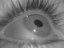
\includegraphics[scale=.6]{imagens/olhos/(2,4).jpg}}\hspace{2pt} \Bigg\vert\hspace{2pt} \raisebox{-9pt}{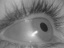
\includegraphics[scale=.6]{imagens/olhos/(4,1).jpg}} \hspace{2pt}\Bigg\vert \cdots \Bigg\vert \hspace{2pt}\raisebox{-9pt}{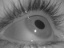
\includegraphics[scale=.6]{imagens/olhos/(6,4).jpg}}\hspace{2pt}  \right]$$

$$y = \left[ \hspace{2pt} \raisebox{-9pt}{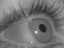
\includegraphics[scale=.6]{imagens/olhos/(5,2).jpg}} \hspace{2pt} \right]$$
\caption{Dada uma matriz com as amostras e uma imagem $y$, identificamos as amostras mais parecidas com $y$ usando o modelo \textit{cross-and-bouquet}, depois estimamos o olhar como a média ponderada das posições de olhar dessas amostras.}
\label{fig:matriz_olho}
\end{figure}

Pelo modelo \textit{cross-and-bouquet}, para cada vetor correspondendo à imagem $y$, calculamos um vetor $x = (c, e)$ tal que $y = Ac + e$. Podemos assumir que as amostras mais parecidas com $y$, são as colunas $a_i$ de $A$ onde $c_i$ possuem maior valor em módulo. Assumindo isso, estimamos a posição do olhar para a imagem $y$ como a média ponderada das posições do olhar das três imagens mais parecidas com $y$, onde $\vert c_i \vert$ são os pesos.

Antes de comparar as imagens usando o modelo \textit{cross-and-bouquet} reduzimos as imagens aplicando a pirâmide gaussiana $3$, $4$ ou $5$ vezes, resultando em imagens $60 \times 80$, $40 \times 30$ e $20 \times 15$, respectivamente. Fazemos isso para evitar erros de memória durante a execução do programa.

\newc{Após calcular a matriz $A$, estimamos o olhar de cada imagem. A entrada do algoritmo será então a imagem e a saída será a posição do olhar em graus do campo de visão do usuário.}

\section{Resultados}
A Tabela $\ref{tab:erros}$ mostra a média dos erros (conhecida como acurácia) e o desvio padrão (a precisão), considerando  diferentes tamanhos de imagens. Podemos observar que o erro é menor se usamos imagens maiores para estimar o olhar. Para imagens $60 \times 80$, obtemos uma acurácia de $1,053 $ e precisão de $2,279$, semelhantes aos resultados obtidos pelo rastreador Tobii EyeX, que tem acurácia de $1,42$ e precisão de $1,70$, segundo \cite{liboku}. \newc{A Tabela $\ref{tab:erros}$ indica também o tempo médio para estimar o olhar em cada imagem.}

\begin{table}
\centering
\begin{tabular}{| c | c | c | c |}
\hline
%& \multicolumn{3}{| c |}{dimensão das imagens} \\ \hline
dimensões das imagens & $15 \times 20$ & $30 \times 40$ & $60 \times 80$ \\ \hline
Erro				  & $1,471 \pm 2,398$ & $1,113 \pm 2,291$ & $1,053 \pm 2,279$ \\ \hline
Tempo de processamento & $0,035s$ & $0,215s$ & $5.311s$ \\ \hline
Imagem & \vspace{2pt} 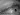
\includegraphics[width=2cm]{imagens/olho_20_15.jpg} & 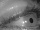
\includegraphics[width=2cm]{imagens/olho_40_30.jpg} & 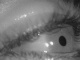
\includegraphics[width=2cm]{imagens/olho_80_60.jpg} \\ \hline
\end{tabular}
\caption{Erros na estimação do olhar para diferentes tamanhos de amostras. Cada coluna representa o tamanho das imagens usadas, e cada célula representa o erro médio $\pm$ o desvio padrão em graus. \newc{Vemos também o tempo médio para estimar o olhar de cada imagem.} A última linha mostra exemplos de imagens usadas nas respectivas dimensões.}
\label{tab:erros}
\end{table}

A Figura $\ref{fig:erros_posicao}$ mostra a distribuição dos erros nos pontos da grade para diferentes tamanhos de imagem, após reduzir as imagens originais aplicando a pirâmide gaussiana $3$ vezes (resultando em uma imagem $60 \times 80$, $4$ vezes (resultando em imagens $30 \times 40$ e $5$ vezes (resultando em imagens $15 \times 20$). Podemos notar na última imagem que os erros são maiores nos cantos da grade.

\begin{figure}
\centering
	\begin{subfigure}[b]{0.4\textwidth}
        \centering
        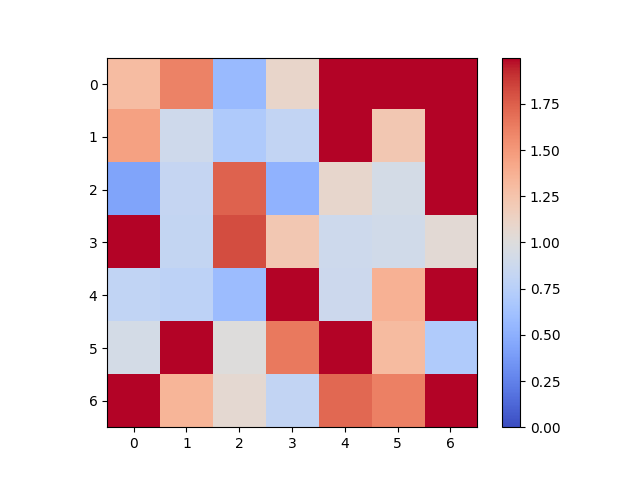
\includegraphics[scale=.4]{imagens/erros5pyrDown.png}
        \caption{}
    \end{subfigure}
    ~
    \begin{subfigure}[b]{0.4\textwidth}
        \centering
        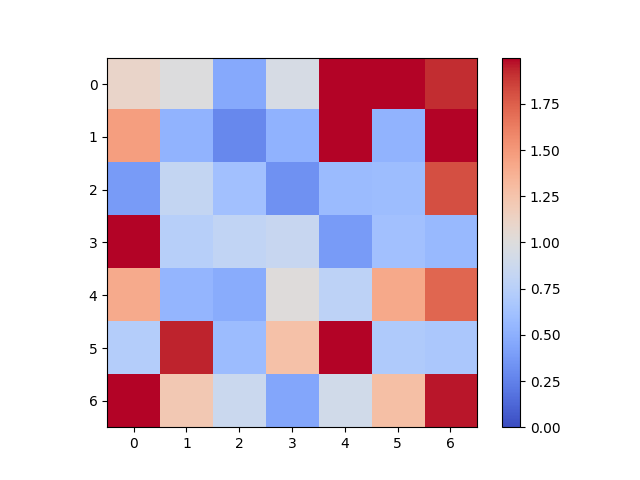
\includegraphics[scale=.4]{imagens/erros4pyrDown.png}
        \caption{}
    \end{subfigure}\\
    
    \begin{subfigure}[b]{0.4\textwidth}
        \centering
        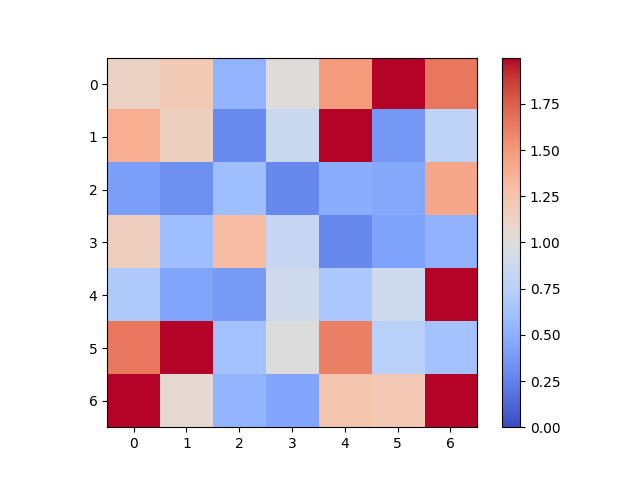
\includegraphics[scale=.4]{imagens/erros3pyrDown.png}
        \caption{}
    \end{subfigure}
        
    \caption{Erros médios para cada posição na grade, usando amostras correspondentes a uma grade $7 \times 7$. Em {\bf (a)} As imagens usadas têm dimensão $20 \times 15$, em {\bf (b)} as imagens são $40 \times 30$ e em {\bf (c)} as imagens são $60 \times 80$.}
    \label{fig:erros_posicao}
\end{figure}

A Figura \ref{fig:erros_participante} mostra a acurácia para cada participante. Observando os dados e as imagens registradas durante o experimento, notamos que se o participante piscar durante a coleta das amostras, o resultado será pior. O participante $2$, por exemplo, piscou algumas vezes durante a coleta de algumas amostras (que eram usadas para estimar o olhar nas outras imagens), acreditamos que por isso o resultado foi pior que os dos outros participantes.

\begin{figure}
    \centering
    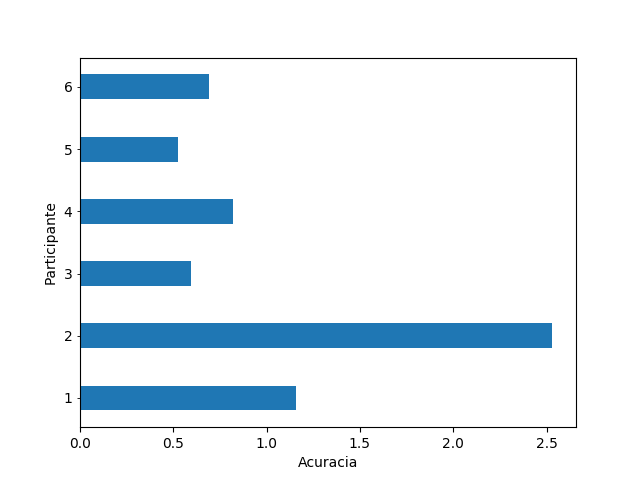
\includegraphics[scale=.6]{imagens/errosParticipantes_pyrDown3.png}
    \caption{A figura mostra a acurácia para diferentes participantes usando o algoritmo para estimar olhar com imagens $60 \times 80$. \newc{A acurácia para o participante $2$ foi pior porque ele piscou durante a coleta das amostras.}}
    \label{fig:erros_participante}
\end{figure}

Uma limitação do experimento foi que todas as imagens correspondentes a um ponto na grade foram coletadas durante um intervalo de um segundo, então elas talvez sejam mais parecidas entre se do que seriam se fossem registradas em momentos diferentes.

Apesar das limitações do experimento, o rastreador apresentou um desempenho semelhante ao de um rastreador comercial.
\chapter{Conclusão}

Neste trabalho estudamos conceitos de rastreamento de olhar, a teoria de \textit{Compressive Sensing}(CS) e desenvolvemos um programa de rastreamento de olhar.

%Observamos que CS é útil tanto para recuperar sinais esparsos, como também para comparar imagens.

CS é útil para recuperar sinais esparsos, resolvendo com alta probabilidade um problema NP. Uma variação do CS pode ser usada para comparar imagens, usamos esta variação para construir um rastreador de olhar.

Elaboramos um experimento para testar a precisão e acurácia do rastreador e notamos que o programa apresenta algumas limitações, por exemplo, o programa não consegue estimar o olhar para determinada região se o participante piscar durante a coleta da amostra correspondente. Apesar das limitações, o experimento apresentou um resultado semelhante ao de um rastreador comercial.

Este trabalho contribuiu para a formação do aluno em Matemática Aplicada pois, durante o ano o aluno estudou a técnica de \textit{Compressive Sensing}, que apresenta resultados não triviais, e a usou em um problema de processamento de imagens.


\appendix
\chapter{Pseudoinversa}


% ---------------------------------------------------------------------------- %
% Bibliografia
%\backmatter \singlespacing   % espaçamento simples
%\bibliographystyle{plainnat-ime} % citação bibliográfica textual
\bibliographystyle{plain}
\bibliography{bibliografia}  % associado ao arquivo: 'bibliografia.bib'

\end{document}
